\label{chap:array_write_process}
This chapter provides the reader with an overview of the data formatting required to drive an IRLED array, and hardware specific details of the underlying array write process to facilitate an understanding of the context in which the PDP is implemented as well as highlight some of the challenges with high-speed operation. Firstly, it discusses the interleaved write process required to directly drive LEDs on an IRLED IRSP. Then, it discusses the data re-ordering done to optimize the write process. Protocol level details of how external data is received are discussed in Chapter~\ref{chap:display_protocols}.


\section{Array Interleaved Write Process}
    \label{sec:array_Interleaved_write_process}
    Although all current IRSP arrays utilize display protocol technology that is decoded pixel by pixel to drive the emitters of an array, arrays may utilize different internal drawing mechanisms for driving pixels. This section discusses the details of those mechanisms within the TCSA, NSLEDS, and HDILED arrays for conceptual purposes, and while the details may differ for other arrays, the overall raster write process is generalizable in the sense that not all pixels are driven at once. Instead some subset of pixels is driven depending on how many analog channels can be utilized at the same time. The number of channels is largely dependent on the array design; however, in some cases the circuitry an array is mounted to allows for some configuration\footnote{Figure~\ref{fig:round_board} shows an example of supporting circuitry in Chapter~\ref{sec:close_support_electronics}}. For example, an HDILED array has 32 channels in typical configurations, meaning that it can drive 32 pixels at once. However, each quadrant can be operated independently with certain board setups, yielding up to a 128-channel maximum. Similarly, it can also be configured to utilize only 16 channels, 8 channels, 4 channels, and 2 channels as well. The details of these configurations are discussed in more detail later in this section.

    Arrays which operate in a snapshot mode also exhibit similar operational behavior. Snapshot mode is a type of array operation in high-speed projector systems in which light output does not occur until every pixel for a frame is written. It works by only transferring charge to embedded emitters once all pixel data is written~\cite{McHughEtAl1999}. This has the benefit of reducing heat variation across an array. However, the actual write process is very similar to non-snapshot operation which is often referred to as a rolling-update mode of operation within literature. Similar to rolling-update operation, each pixel charges either individually or in segments. The only difference is that the emitters themselves are enabled later. The write order and number of pixel segments driven at the same time is array dependent though.

    The TCSA, NSLEDS, and HDILED arrays are organized into four quadrants as shown in Figure~\ref{fig:tcsa_nsleds_hdiled_quads}. Each quadrant is organized into a given number of pixels with TCSA housing 256 by 256, NSLEDS housing 512 by 512, and HDILED housing 1024 by 1024 per quadrant. There are number of input signals necessary to drive an array. These are {\em a 4-bit quadrant write enable}, {\em X address}, {\em Y address}, {\em LOAD bit}, {\em 16 Strong/Weak drive strength bit}, {\em array reset bit}, and {\em analog signaling lines which charges the pixels being addressed}. The quadrant write enable, X address, Y address, and LOAD signals are all utilized for addressing the array.

    \begin{figure}
        \centering
        %includegraphs[trim=L B R T]
        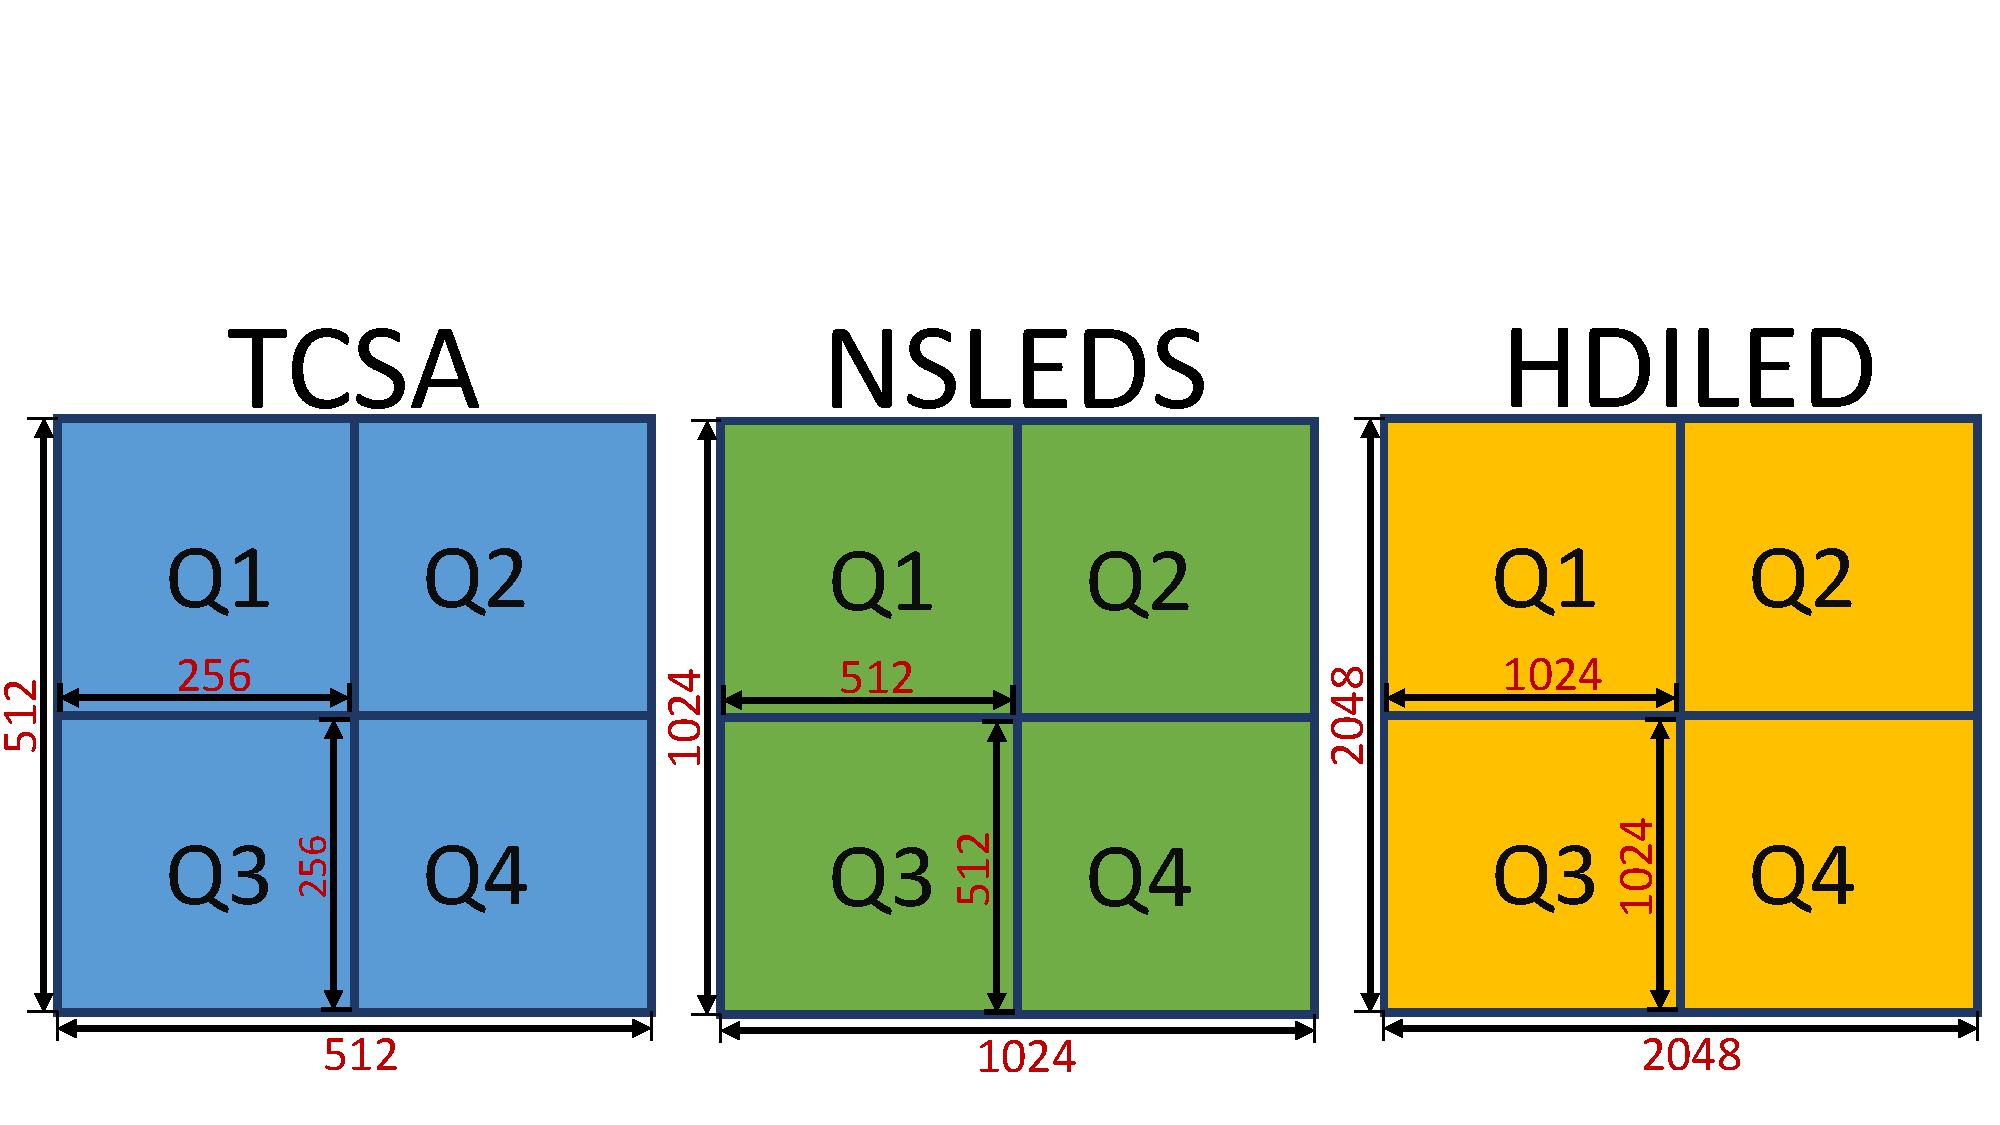
\includegraphics[width=1.0\textwidth]{fig/tcsa_nsleds_hdiled_quads.pdf}
        \caption[TCSA, NSLEDS, and HDILED Array Quadrant Layouts]{TCSA, NSLEDS, and HDILED Array Quadrant Layouts\textsuperscript{a}}
        \vspace{0px}
        \footnotesize\textsuperscript{a} Not drawn to scale
        \label{fig:tcsa_nsleds_hdiled_quads}
    \end{figure}

    The quadrant write enable selects which quadrant to drive. It is worth noting that each quadrant has separate internal signaling which allows for each quadrant to operate independently in parallel when mounted in a package that provides independent external signals as noted earlier. However, to date most of the fabricated IRLED arrays are mounted in packages that allows for only one quadrant to be drawn at a time. At the time of writing, only HDILED has been tested in the type of setup~\cite{LassiterEtAl2019_0, LassiterEtAl2019_1, LassiterEtAl2019_2, LassiterEtAl2020} due to it having the largest resolution per quadrant. During independent quadrant operation, multiple independent CSEs must be utilized. In a two CSE setup, half of the quadrant bits would be controlled by one CSE and half by another. This would yield a total of 64 channels being written in parallel for double the analog performance. In a four CSE setup, a single quadrant would be controlled by a single CSE. This would yield a total of 128 channels being written in parallel for quadruple the analog performance. Irrespective of the number of CSEs used to a drive an array, the internal RIIC signal lines would be driven in precisely the same manner within each quadrant with the only change being that they operate asynchronously with respect to the others.

    The X address, Y address, and LOAD are used to select which pixel or group of pixels to write within a quadrant depending on the mode of operation. Though these lines are effectively shared by quadrants in a single CSE Setup, within the RIIC architecture they can be driven independently to enable the multiple CSE operation mentioned previously. Internally, each array (or quadrants in multi-CSE setups) can write up to 32 pixels (or channels) of data at a given time. As noted previously, the mode of operation dictates whether 2, 4, 8, 16, or 32 channels are used. It also affects the number of address bits utilized in practice with lower modes of operation using more bits. Additionally, the number of address bits differs by array due to the differences in sizes. NSLEDS utilizes 7 bits for the X address and 7 bits for the Y address, yielding a total of 256 by 256 addresses per quadrant. The LOAD bit is used to select between even and odd rows, yielding an effective address space of 256 by 512 per quadrant. Because the smallest mode of operation writes 2 pixels at a time, this is sufficient to fully address the array. Similarly, HDILED utilizes 8 bits for the X address and 8 bits for the Y address, yielding a total of 512 by 512 addresses per quadrant. Again, as with NSLEDS, the LOAD bit is used to select between even and odd rows, yielding an effective address space of 512 by 1024 per quadrant. This is again sufficient to completely address the array since it also can at a minimize write 2 pixels at a time.

    Structurally, NSLEDS and HDILED are laid out as super pixel as shown in Figure~\ref{fig:nsleds_hdiled_array_superpixel_layout}. Each super pixel is made up of a grid of 4 pixels spanning two rows and columns. These are laid out across the array in a grid structure with NSLEDS consisting of 256 by 256 super pixels, and HDILED consisting of 512 by 512 super pixels. This image also highlights two points discussed above, the LOAD line selects between the top two pixels (even rows) and bottom two pixels (odd rows) of each super pixel in the quadrant, and the two selected pixels are both written at the same time. Additionally, these share a drive strength as noted in the diagram. This is controlled using the Strong/Weak drive strength bits which dictate whether to provide a strong or weaker light emission for the given pair of pixels.

    \begin{figure}
        \centering
        %includegraphs[trim=L B R T]
        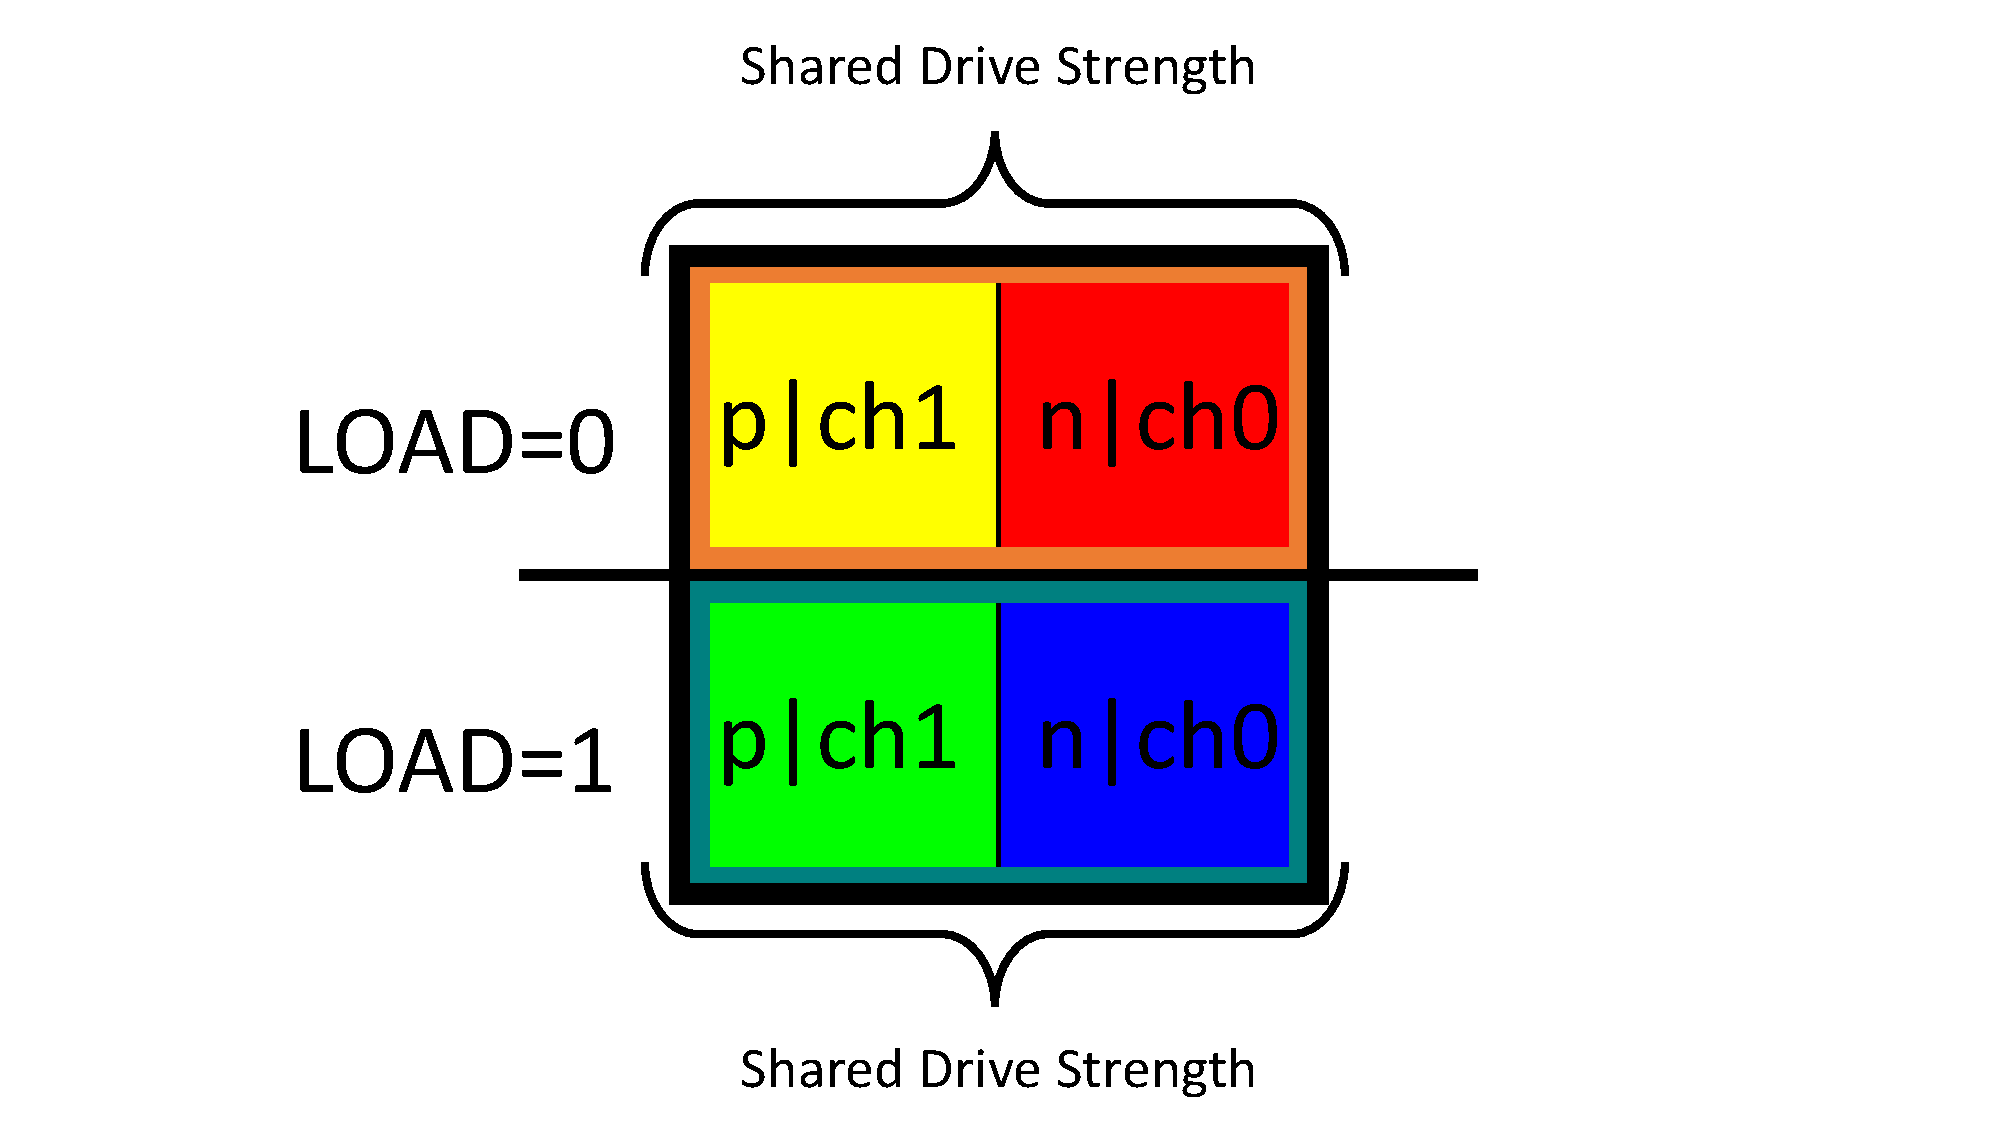
\includegraphics[width=0.50\textwidth]{fig/superpixel_layout.pdf}
        \caption{NSLEDS/HDILED Array Super Pixel Layout}
        \label{fig:nsleds_hdiled_array_superpixel_layout}
    \end{figure}

    The 32 analog signaling lines control the emission intensity of driven pixels. These 32 channels are controlled by digital to analog converters within the CSE that are driven by the firmware. Internally, a CSE has 8 DAC cards with 2 DAC integrated circuits per card, with each DAC circuit consisting of 2 DAC channels as discussed in Chapter~\ref{sec:close_support_electronics}. Each channel is used to drive a single pixel, giving the ability to drive 32 pixels at once or some subset as mentioned previously.

    In practice, it is preferable to utilize all channels at once because this allows for more pixels to be driven in a shorter amount of time. Each of the lower modes of operation cut analog bandwidth in half each time the channel count is halved. Figure~\ref{fig:nsleds_hdiled_array_interleaved_pixel_mapping_per_write} shows the pixel mapping per write for 32 physical pixels on an array in the highest mode of operation. 2 by 32 columns of pixels are shown segmented into super pixels. The Y address denotes the 16 super pixels that are selected per address. If the {\it Y Address} is incremented by 1 then the next 16 rows of super pixels would be selected. The {\it X address} (not shown) simply selects the next column of super pixels. {\it DAC Card} denotes which DAC card drives the given super pixel. {\it L} denotes which value of LOAD will select which rows within each super pixel. When LOAD is low as shown in the middle segment, the top pixels of a superpixel are selected as indicated in cyan. When LOAD is high as shown in the right segment, the bottom pixels of a superpixel are selected.

    \begin{figure}
        \centering
        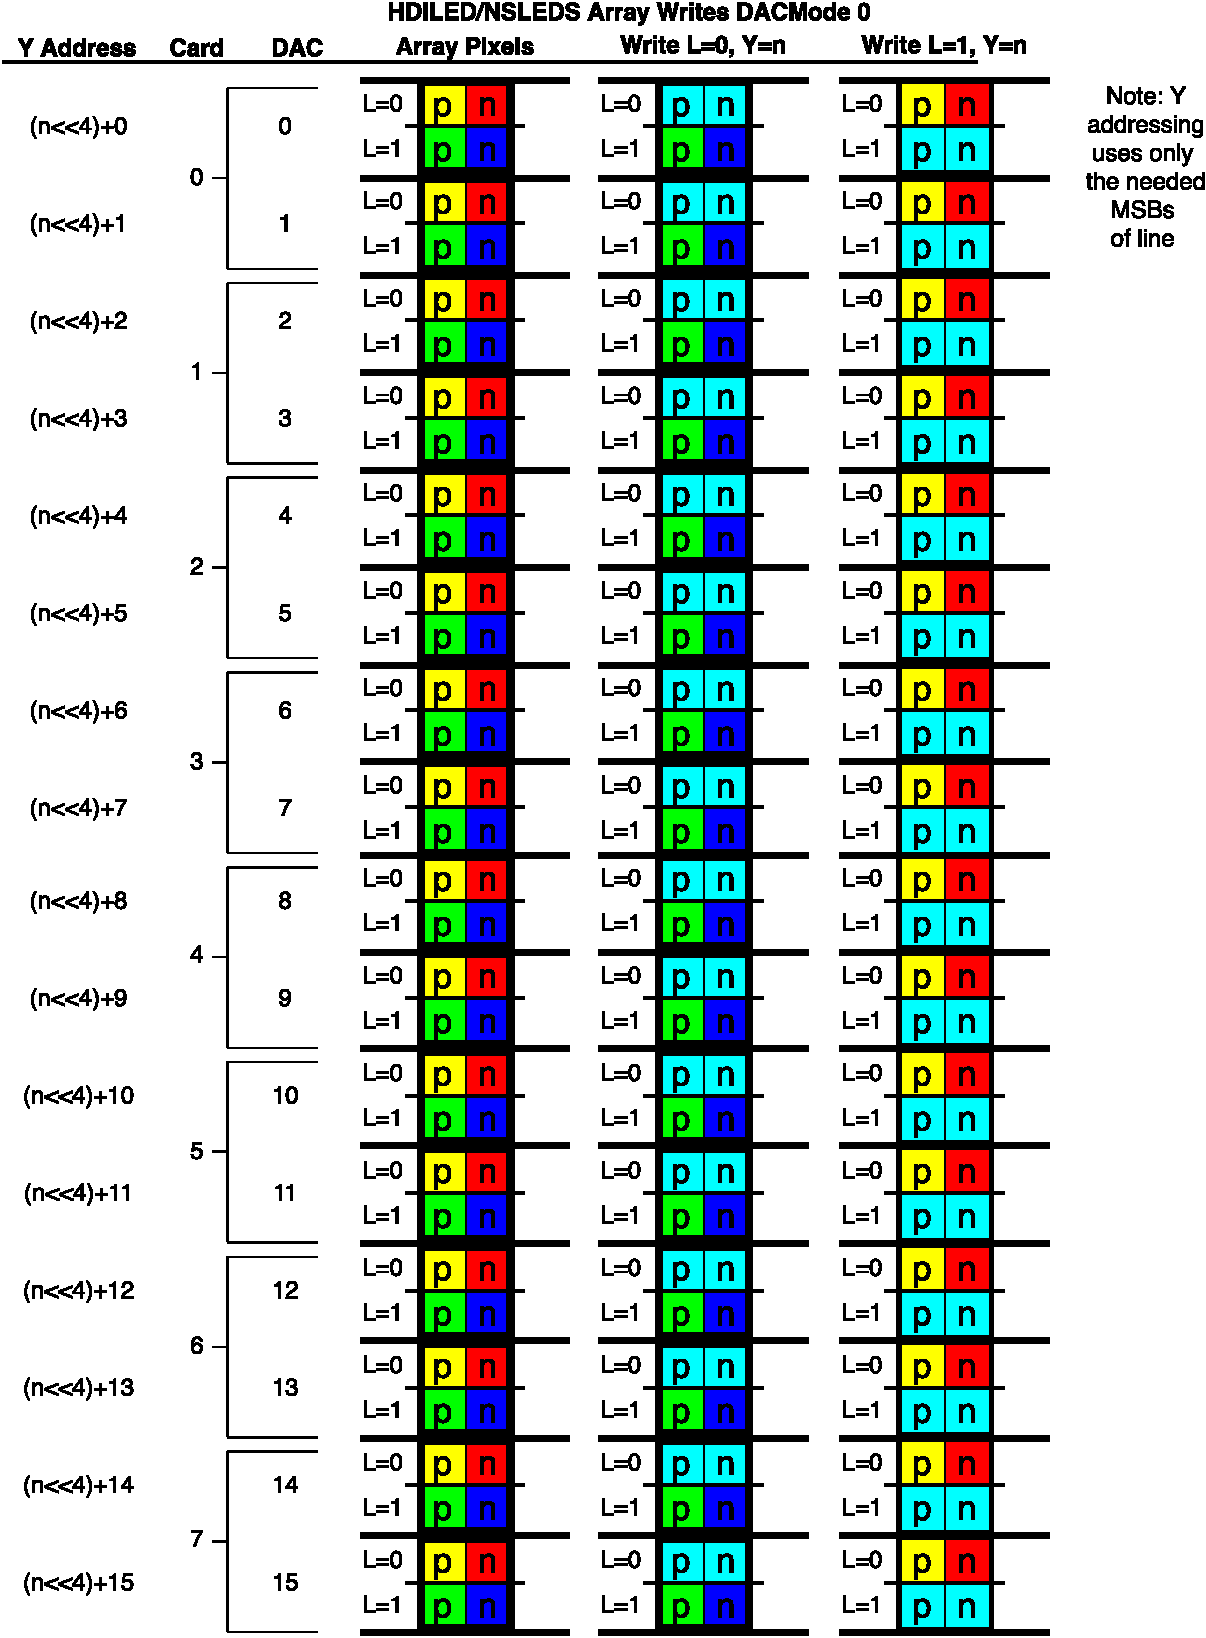
\includegraphics[width=0.98\textwidth]{fig/nsleds_hdiled_array_writing.pdf}
        \caption{NSLEDS/HDILED Array Interleaved Pixel Mapping Per Write}
        \label{fig:nsleds_hdiled_array_interleaved_pixel_mapping_per_write}
    \end{figure}

    The overall writing process for writing 64 pixels is a two-step process. First, 32 values for the even rows are loaded in and written to the array, followed by 32 values from the odd rows being loaded in and written to the array. At a data level, it is ideal to interleave the data such that it is available at the optimal time to reduce latency and buffering requirements within the firmware. This is discussed in detail in Chapter~\ref{chap:pdp_protocol}.

    Writing additional segments of pixels is simply a matter of buffering more data and repeating the same write process while asserting the correct address lines for each segment. Given that arrays have no inherit hardware required write order other than what has been discussed above, the exact order of writing independent segments of 32 pixels can change depending on a number of factors. In a single CSE Setup, under most circumstances, the data for the top quadrants is carried by a single HDMI input going into a CSE, and the data for the bottom quadrants carried by the other HDMI input\footnote{As will be discussed in Chapter~\ref{chap:implementation} when utilizing the PDP for driving an array, the location of where data is written to an array is agnostic to the HDMI input the data is transported on.}. In this case, the CSE firmware will swap between writing segments of 32 or 64 pixels to the top and bottom halves of an array. The former if it is desirable to write a minimal amount of data before servicing data from another input, the latter if it is desirable to complete an entire chunk of pixels. In a two CSE Setup, data over the HDMI links data could be segmented either horizontally or vertically meaning that each HDMI link would carry data for an entire quadrant. In a four CSE setup, each link would carry half of the data for a quadrant. As the reader may imagine, the order of writes could be configured in many different ways under these scenarios. Though it will not be discussed in detail within this dissertation, it is worth noting for posterity that the order of writes on IRLED arrays can and does affect the thermal load on an array which ultimately can effect pixel brightness~\cite{BarakhshanEtAl2017, LaVeigneSieglinger2012, Norton2013}; thus, controlling the order of writes can be an important factor to consider for designers and users of a system. As mentioned previously, many of these effects can be alleviated through a snapshot mode operation.

\section{Data ordering}
    \label{sec:data_ordering}
    Due to the interleaved write process described in Chapter~\ref{sec:array_Interleaved_write_process}, data sent to an array is reordered in a manner that simplifies firmware development and minimizes buffering requirements. Though the details of the PDP itself are discussed in later chapters, data ordering is discussed here to illustrate some performance considerations with array operation, and could be considered independent of the PDP in that the data ordering could be implemented in non-PDP firmware.

    Figure~\ref{fig:bit_packing} shows the data bit packing utilized within the system when the PDP is in use. It is designed to map to the superpixel layout shown in Figure~\ref{fig:nsleds_hdiled_array_superpixel_layout}. Shown is a 24-bit pixel word which normally represents an RGB value in RGB color space within display protocols where 8 bits are reserved for each of the red, green, and blue channels. Below this is the mapping of each bit value for an NSLEDS or HDILED array. Where {\it S} indicates the drive strength of the super pixel, {\it L} indicates the value to drive the left side of the super superpixel at, and {\it R} indicates the value to drive the right side of the superpixel at. Only 11 bits are currently used to transmit data per pixel due to bit resolution limitations in the DAC and amplifier boards used within a CSE. Future CSEs may have higher bit resolutions resulting in the need to transmit 16-bits per pixel. In this event bit packing would not be used. There has been some work on improving the DAC architecture as well~\cite{EjzakEtAl2019}.

    \begin{figure}
        \centering
        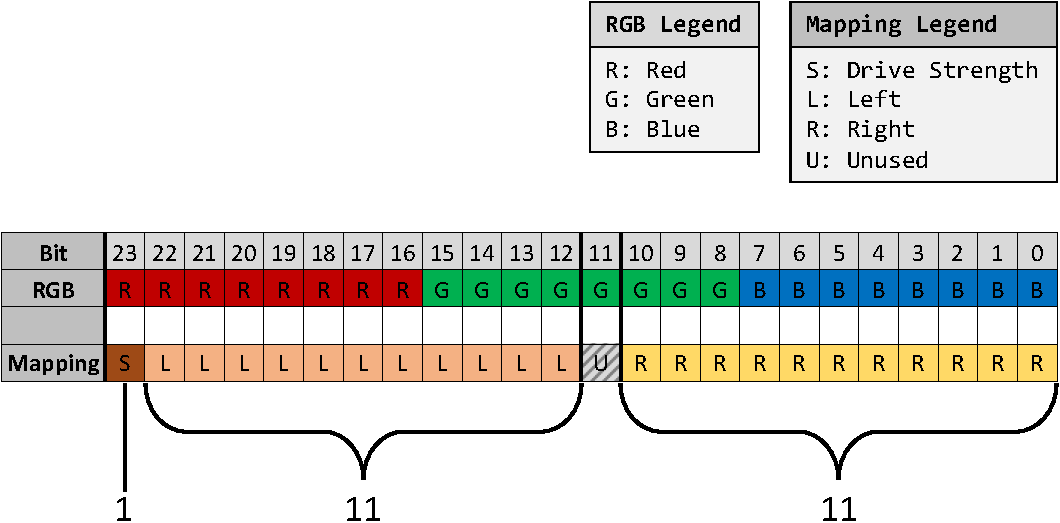
\includegraphics[width=1.0\textwidth]{fig/bit_packing.pdf}
        \caption{Bit-packing Format}
        \label{fig:bit_packing}
    \end{figure}

    Figure~\ref{fig:image_encoding} shows the input reordering performed on data sent to a CSE. Each cable sends half of the data as noted in Chapter~\ref{sec:close_support_electronics}. The input example is segmented into top, middle, and bottom to indicate which part goes over which input and the different reordering steps. The portions denoted as {\it Top} are transmitted over CSE input 1. The portions denoted as {\it Bottom} are transmitted over CSE input 2. The portions marked {\it Middle} are split evenly over both inputs evenly. The first step of data reordering is to bit pack into 11-bit words as shown in Figure~\ref{fig:bit_packing}. Next, even/odd reordering is performed to reduce latency and buffering constraints as will be shown in more detail in subsequent figures. Note the pattern introduced on the words in the diagram due to even/odd reordering. Finally, data is transposed before being sent to the array to accommodate the column write order of the array shown in Figure~\ref{fig:nsleds_hdiled_array_interleaved_pixel_mapping_per_write}. If data were not transposed, then multiple lines of data would need to be buffered to draw 32 pixels for a single write. In fact, the first generation of firmware utilized on the TCSA and NSLEDS arrays required full image buffering before displaying a single pixel on an array which resulted in an entire frame of latency during operation. The second generation of firmware~\cite{HouserEtAl2018} utilized on TCSA, NSLEDS, and HDILED drastically reduced buffering and latency requirements through data reordering, but
    required double the amount of buffering to that of the current implementation of the PDP because it did not have an even/odd row reorder step during encoding. This meant that 2 by 64 pixels of even and odd rows of data were required to be buffered before a single write could occur even though only 2 by 32 pixels are needed by the hardware for a single write. It is worth noting that as mentioned in Chapter~\ref{sec:array_Interleaved_write_process}, different arrays could have different rasterization processes, and in that event the transformations described here would need to be changed to minimize buffering for those scenarios.

    \begin{figure}
        \centering
        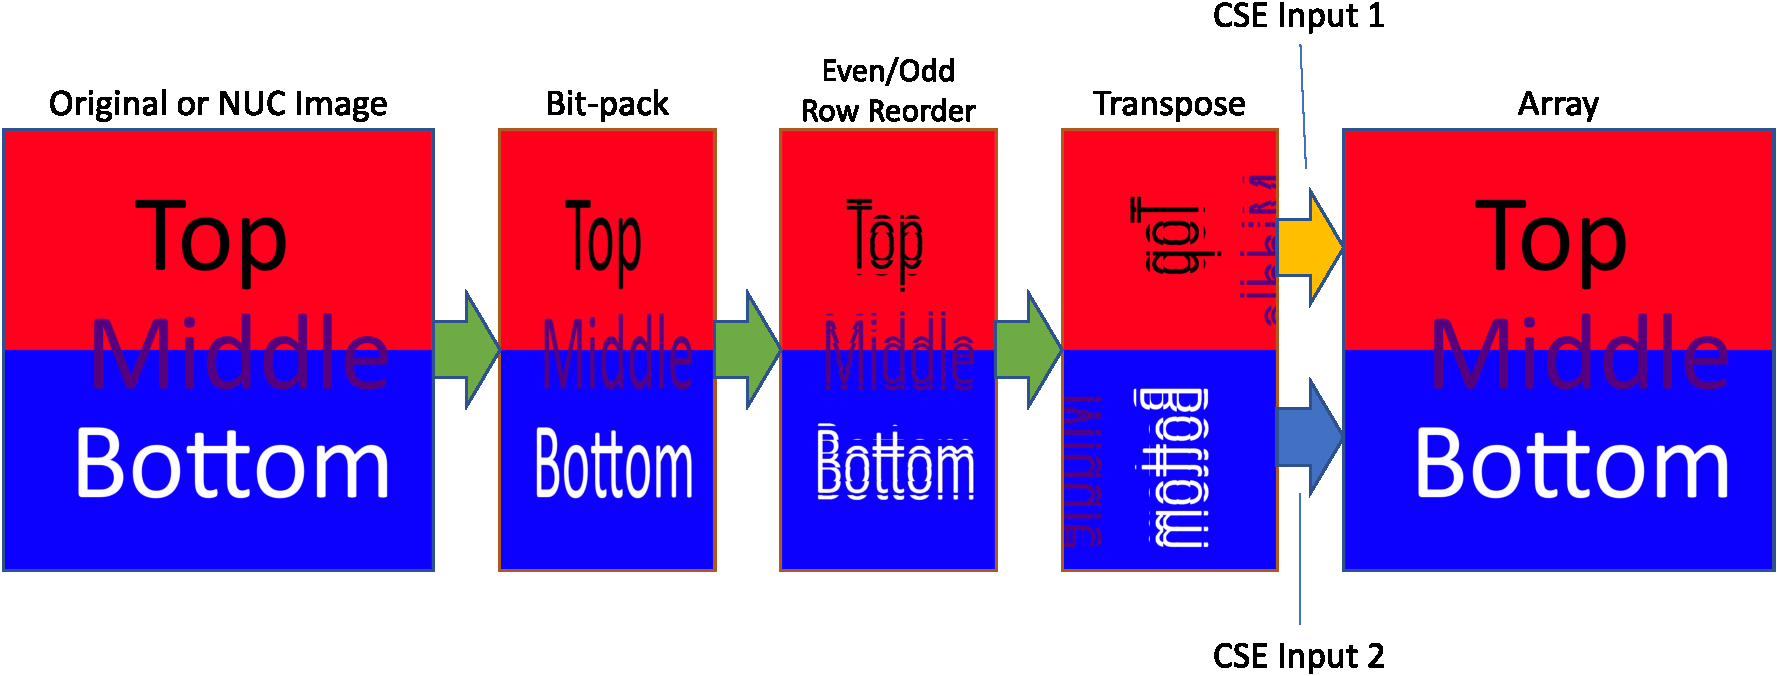
\includegraphics[width=1.0\textwidth]{fig/image_encoding.pdf}
        \caption{Image Encoding: Input Reordering}
        \label{fig:image_encoding}
    \end{figure}

    Figure~\ref{fig:image_encoding_quads} shows how the same image data maps to each quadrant on an array. Similarly, to the previous image the separation of top, middle, and bottom by input cable holds here. Additionally, shown is that quadrant one and two are transmitted over the first input and quadrant three and four over the second input. Note also that the top-left of the image corresponds to quadrant one, the top-right of the image corresponds to quadrant two, the bottom-left of the image corresponds to quadrant three, and the bottom-right of the image corresponds to quadrant four. This relationship holds for all subsequent images. Figure~\ref{fig:image_encoding_colored} shows the same details in a color overlayed chart.

    \begin{figure}
        \centering
        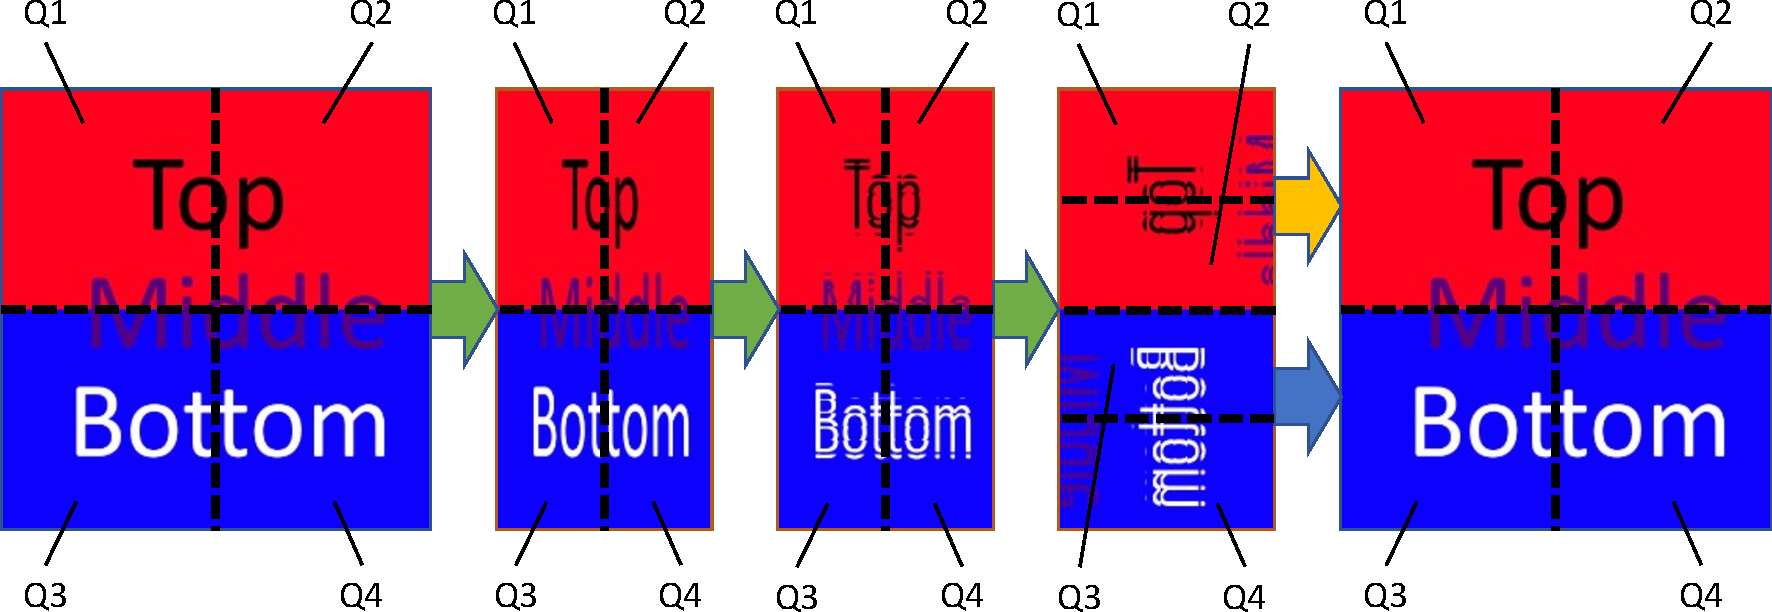
\includegraphics[width=1.0\textwidth]{fig/image_encoding_quads.pdf}
        \caption{Image Encoding: Quadrant Reordering}
        \label{fig:image_encoding_quads}
    \end{figure}

    \begin{figure}
        \centering
        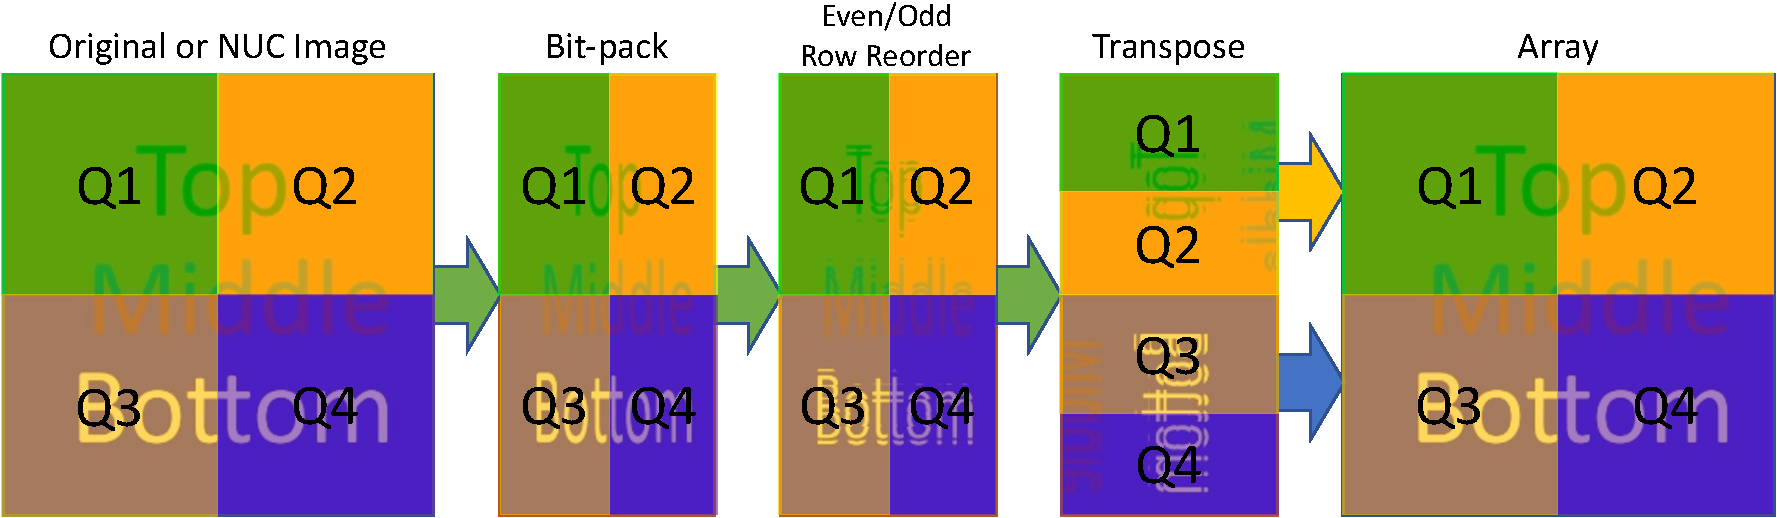
\includegraphics[width=1.0\textwidth]{fig/image_encoding_colored.pdf}
        \caption{Image Encoding: Quadrant Reordering with Color Overlay}
        \label{fig:image_encoding_colored}
    \end{figure}

    Figure~\ref{fig:image_encoding_bitback} shows the bit-packing process for a false color image to aid with understanding. The blown-up sections show single columns of data and the corresponding bit packed version of the data where two columns of input with different colors of data per column are merged into a single column of 24-bit data with one color. This results in the example input image having two solid colors after bit-packing. In the actual implementation of bit packing, real data is in the IR-spectrum and not averaged in this way but clamped and scaled instead. While not required, generally IR data is normally 16-bits per pixel which corresponds to current higher-class IR detectors having a dynamic range of 14-bits per pixel~\cite{FLIR2014_1, FLIR2014_2, FLIR2016}. Cheaper detectors may only have lower dynamic ranges resulting in a lower ability to differentiate light output. Even/odd reordering and the transpose do not result in any noticeable data changes for this example.

    \begin{figure}
        \centering
        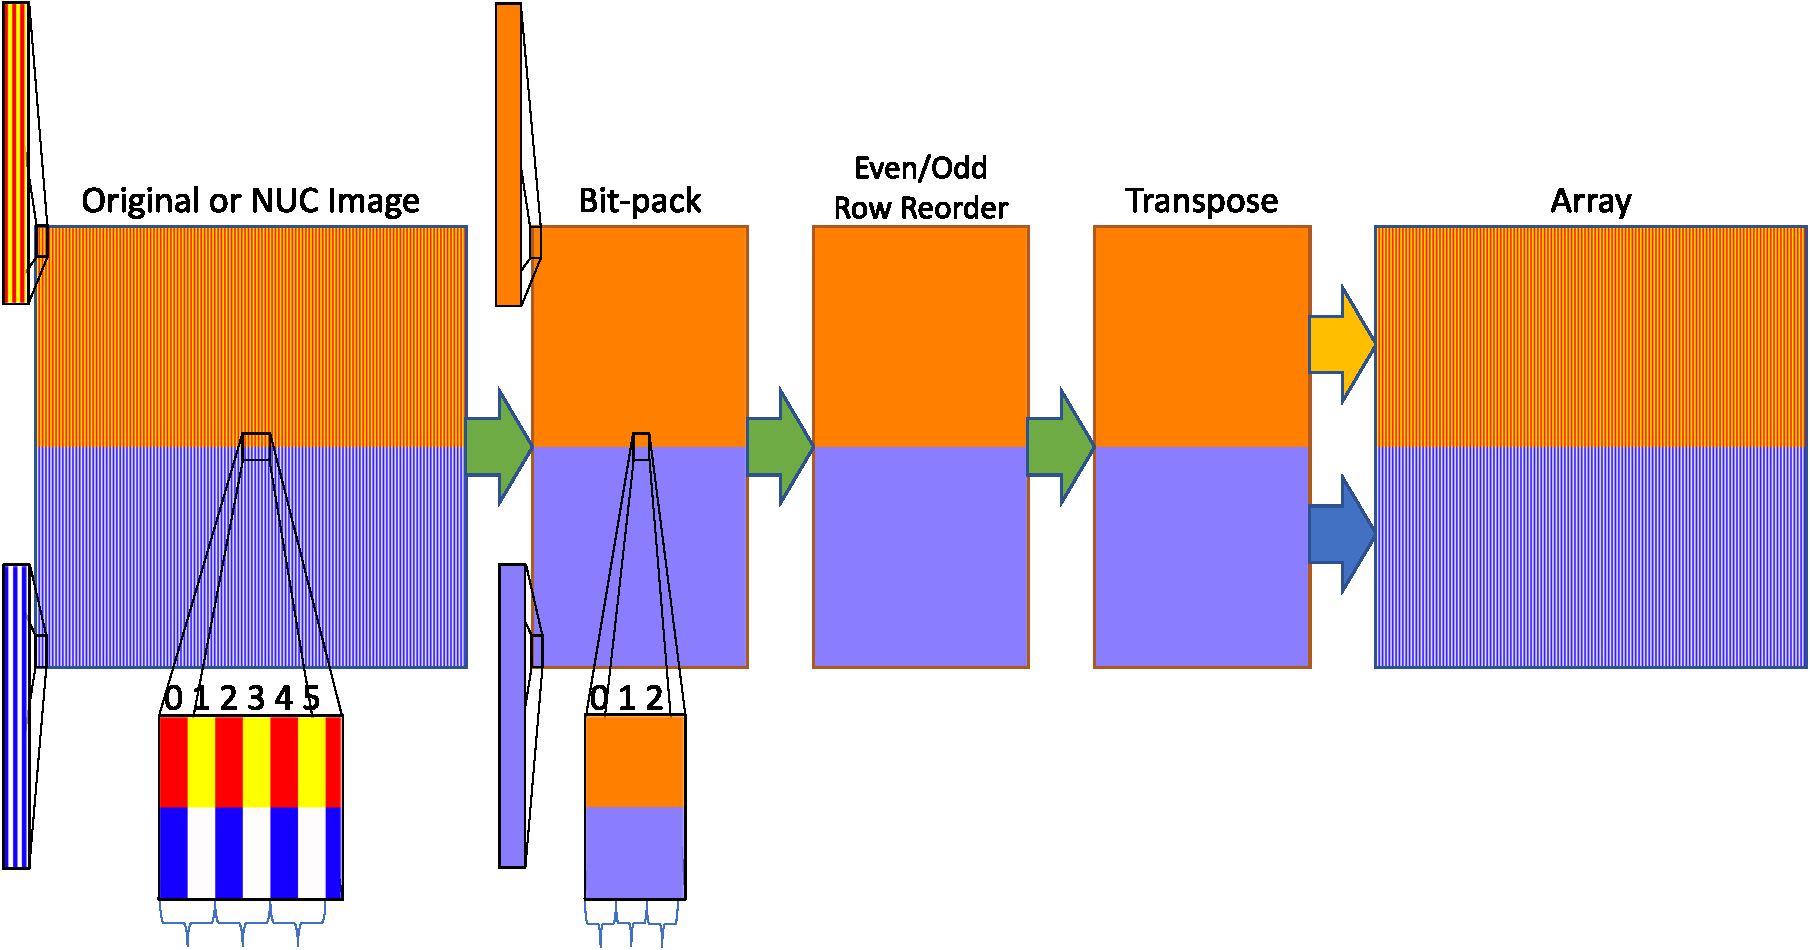
\includegraphics[width=1.0\textwidth]{fig/image_encoding_bitback.pdf}
        \caption{Image Encoding: Data Bit Packing}
        \label{fig:image_encoding_bitback}
    \end{figure}

    Figure~\ref{fig:image_encoding_bitpack_reorder} shows a false color input image designed to highlight the even/odd row reordering applied to imagery. The blown-up sections show 64 labeled rows of input data where the even rows are one color and the odd rows another color for every 32 rows. Additionally, for every 32 rows, the even and odd rows are de-interlaced into 16 even rows of data follow by 16 odd rows of data. In the example input image this results in every 16 de-interlaced rows having a different color. This is due to the interleaved write process for individual 32-pixel writes discussed in Chapter~\ref{sec:array_Interleaved_write_process}. Reordering data allows for only 16 bit-packed pixels of data to be buffered per write. As discussed previously, without this reordering, double the number of pixels would need to be buffered per array write increasing both latency and implementation complexity.

    \begin{figure}
        \centering
        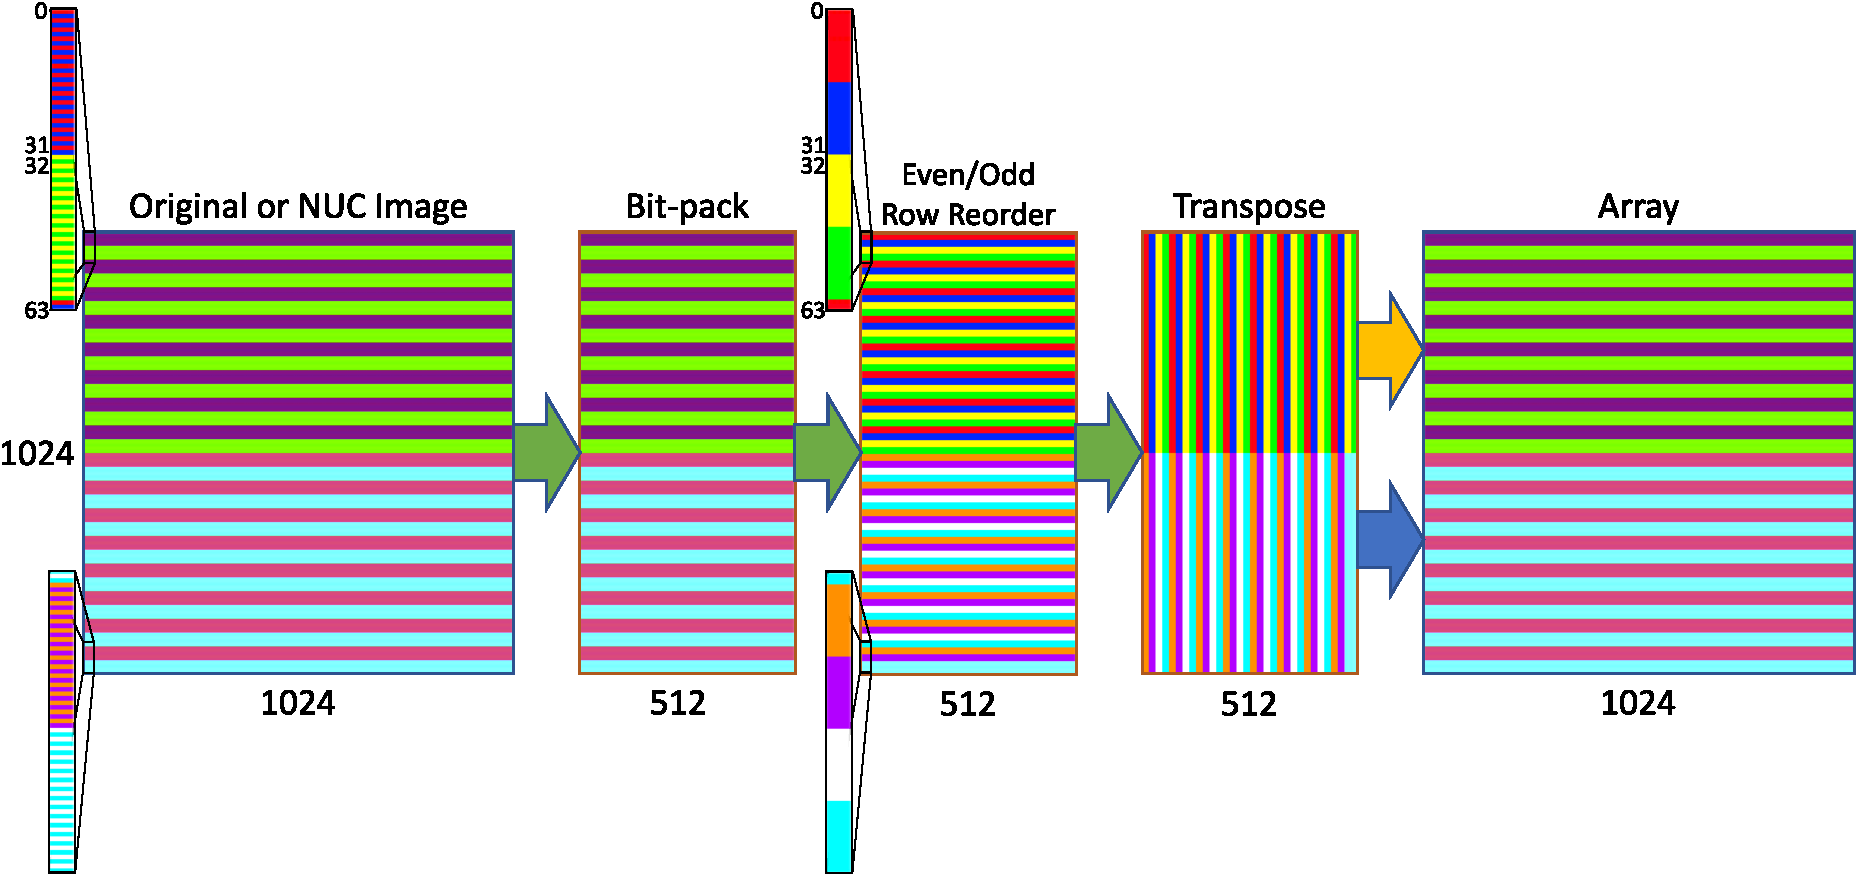
\includegraphics[width=1.0\textwidth]{fig/image_encoding_reorder.pdf}
        \caption{Image Encoding: Data Reorder}
        \label{fig:image_encoding_bitpack_reorder}
    \end{figure}

    Figures~\ref{fig:image_encoding_color_example1},~\ref{fig:image_encoding_color_example2},~and~\ref{fig:image_encoding_color_example3} show some examples of what false colored images would look like if processed by the reordering kernels to give the reader a better understanding of how different types of data would look during the intermediate processes. Note the characteristic jagged pattern due to even/odd row reordering present in each image. Also note that each image is transposed and segmented in half for transfer over separate inputs to a CSE.

    \begin{figure}
        \centering
        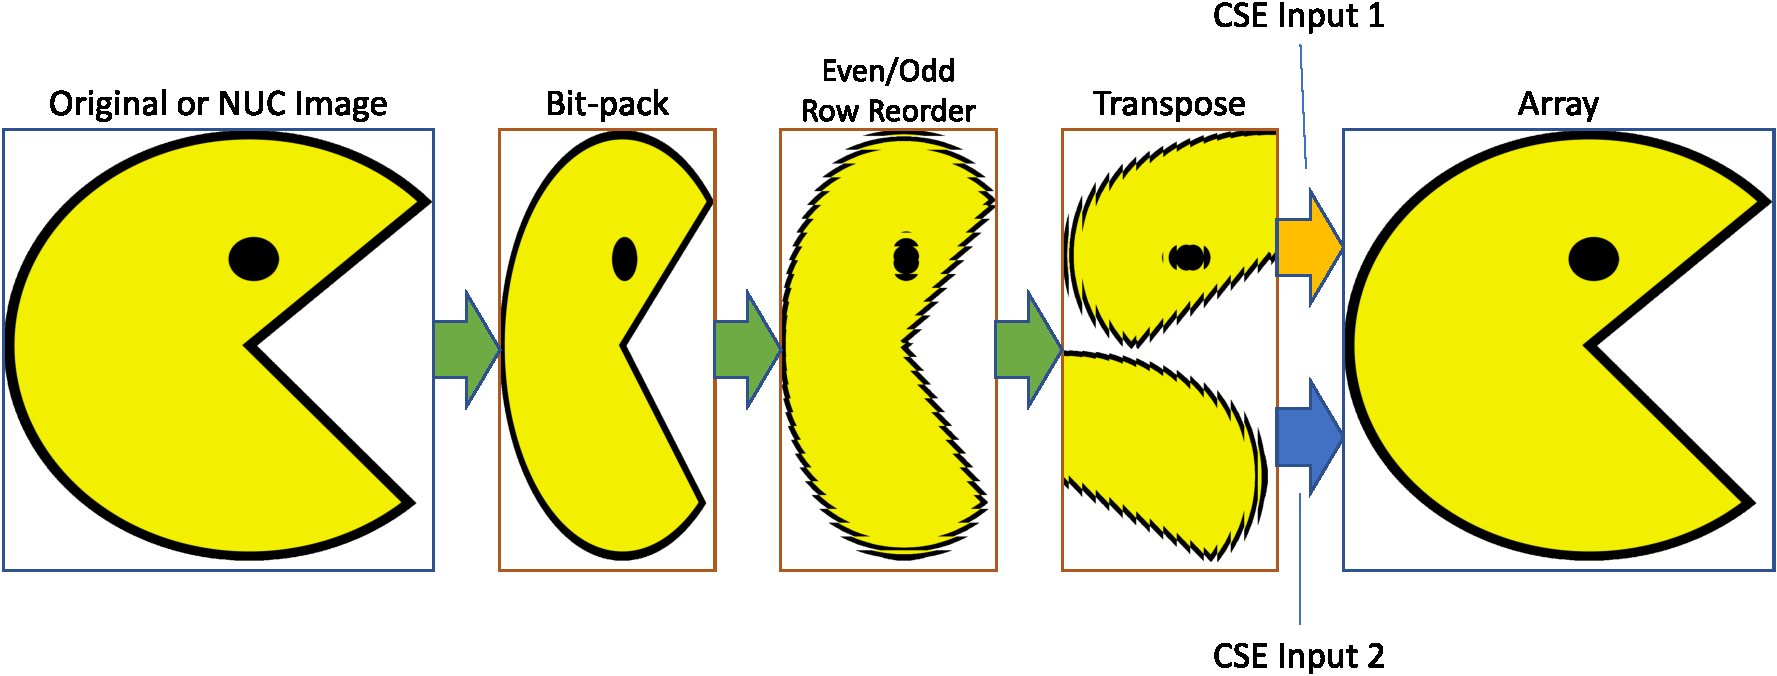
\includegraphics[width=1.0\textwidth]{fig/image_encoding_pac.pdf}
        \caption{Image Encoding: Color Example 1}
        \label{fig:image_encoding_color_example1}
    \end{figure}

    \begin{figure}
        \centering
        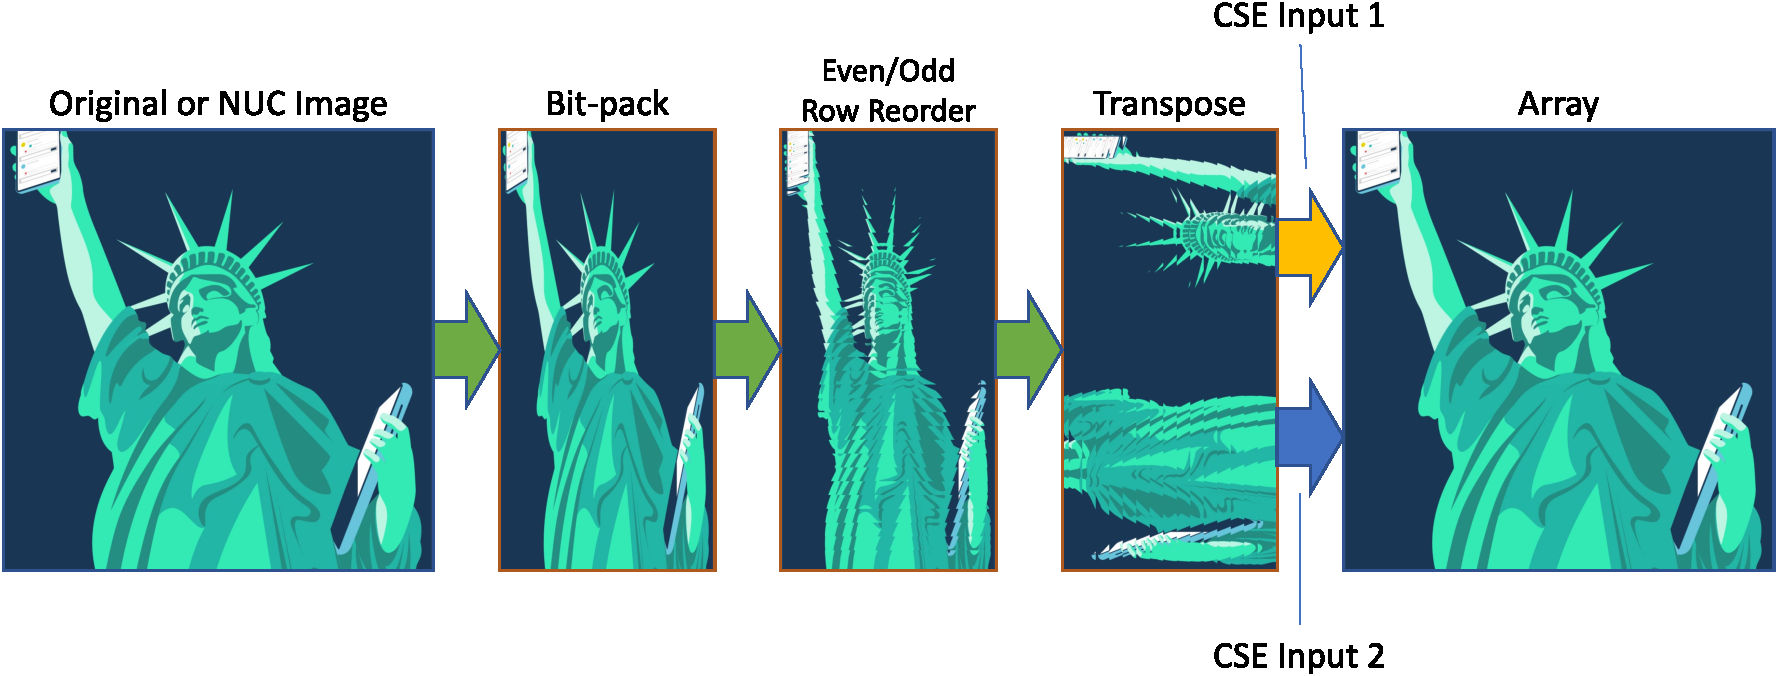
\includegraphics[width=1.0\textwidth]{fig/image_encoding_liberty.pdf}
        \caption{Image Encoding: Color Example 2}
        \label{fig:image_encoding_color_example2}
    \end{figure}

    \begin{figure}
        \centering
        %includegraphs[trim=L B R T]
        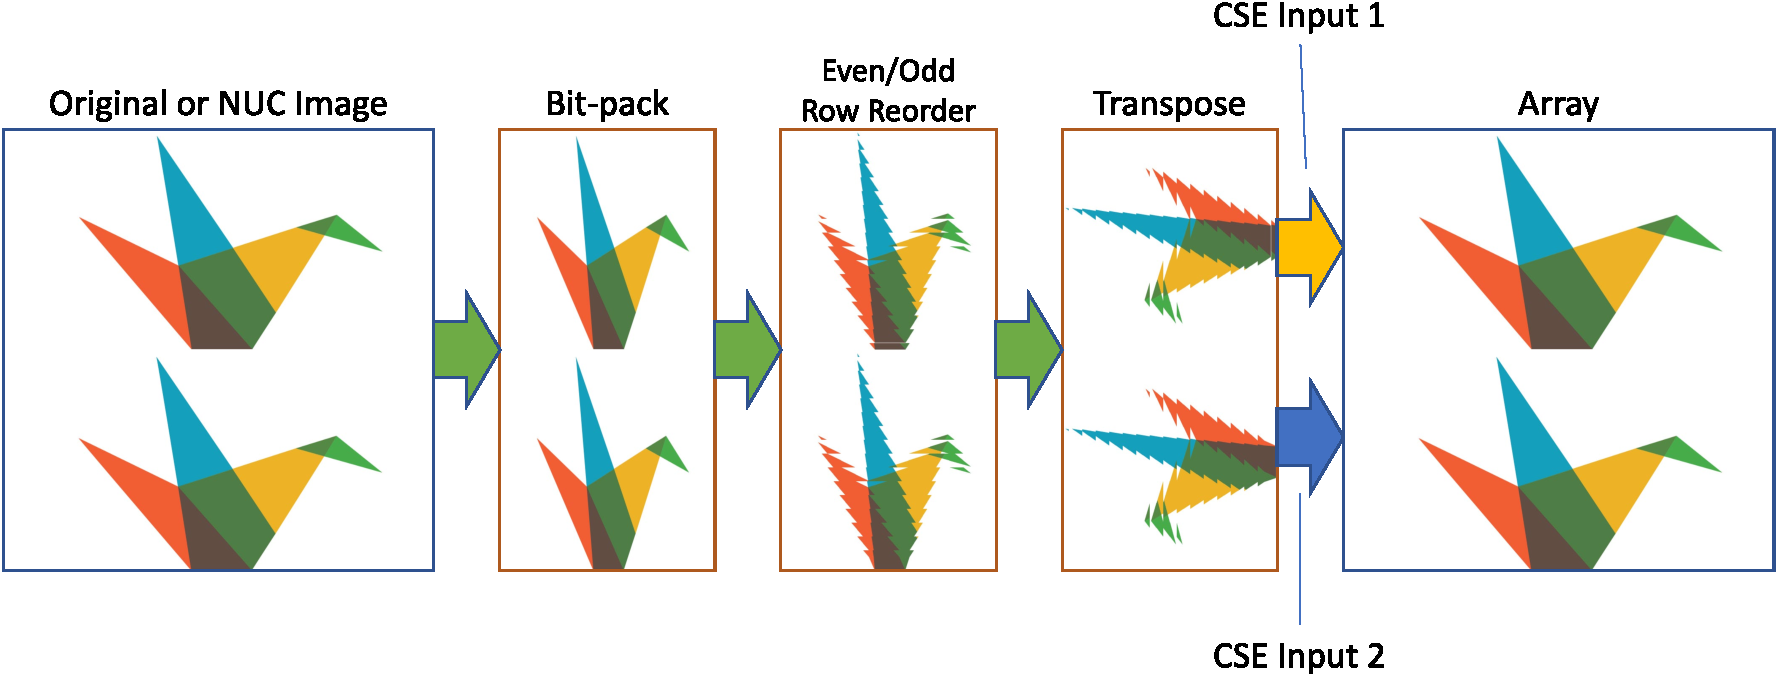
\includegraphics[width=1.0\textwidth]{fig/image_encoding_origami.pdf}
        \caption{Image Encoding: Color Example 3}
        \label{fig:image_encoding_color_example3}
    \end{figure}

    Figures~\ref{fig:image_encoding_ir_example1},~and~\ref{fig:image_encoding_ir_example2} show IR imagery going through the process of reordering. The image shown in Figure~\ref{fig:image_encoding_ir_example1} is commonly used to focus IR cameras and for testing IR array behavior with various shapes and numbers. The image shown in Figure~\ref{fig:image_encoding_ir_example2} is test imagery from one of the projects of my lab. Similarly, to the false color images, images are transposed and sent in halves over the CSE inputs.

    \begin{figure}
        \centering
        %includegraphs[trim=L B R T]
        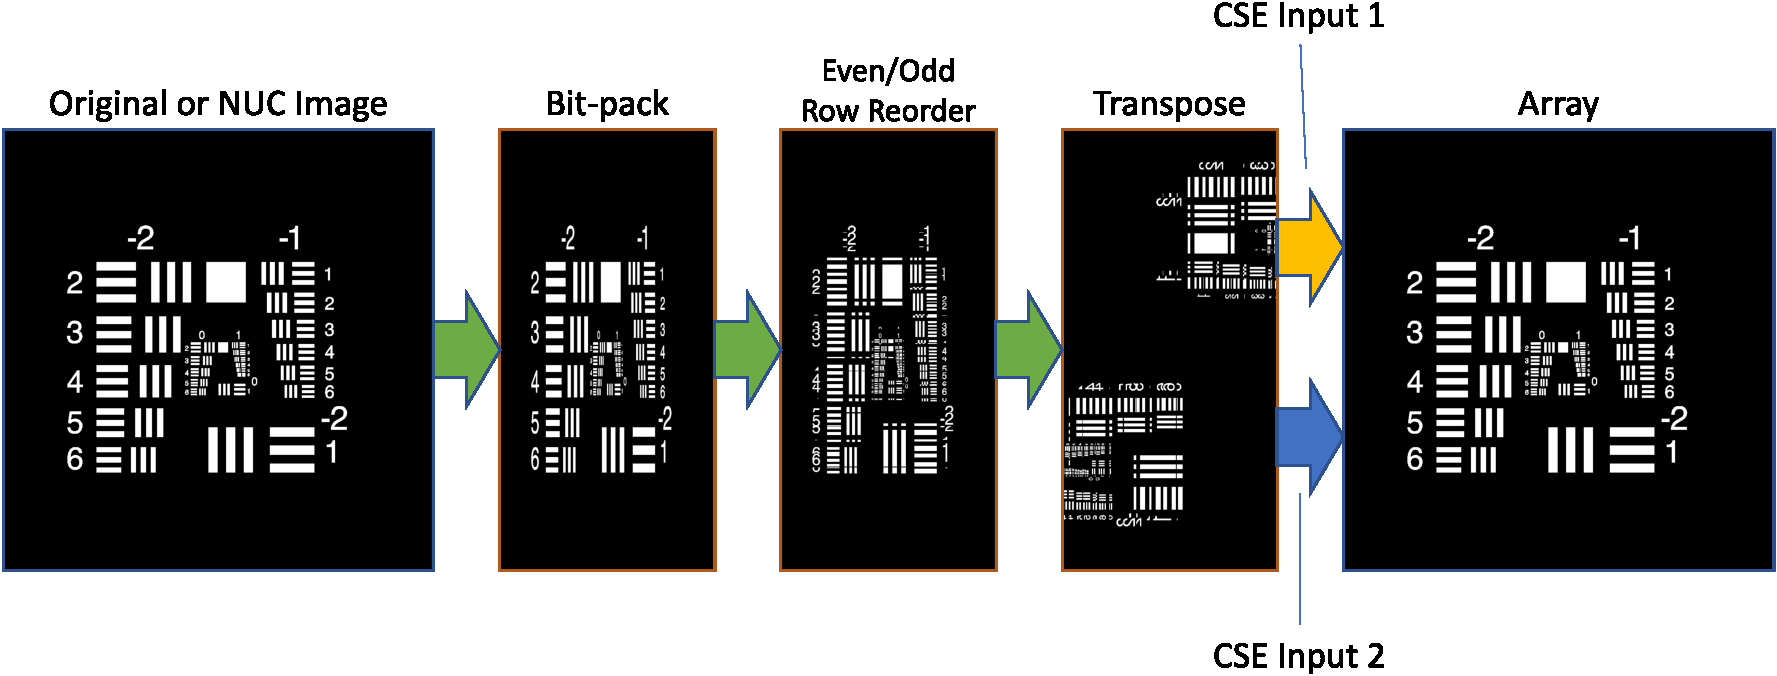
\includegraphics[width=1.0\textwidth]{fig/image_encoding_ir1.pdf}
        \caption{Image Encoding: IR Example 1}
        \label{fig:image_encoding_ir_example1}
    \end{figure}

    \begin{figure}
        \centering
        %includegraphs[trim=L B R T]
        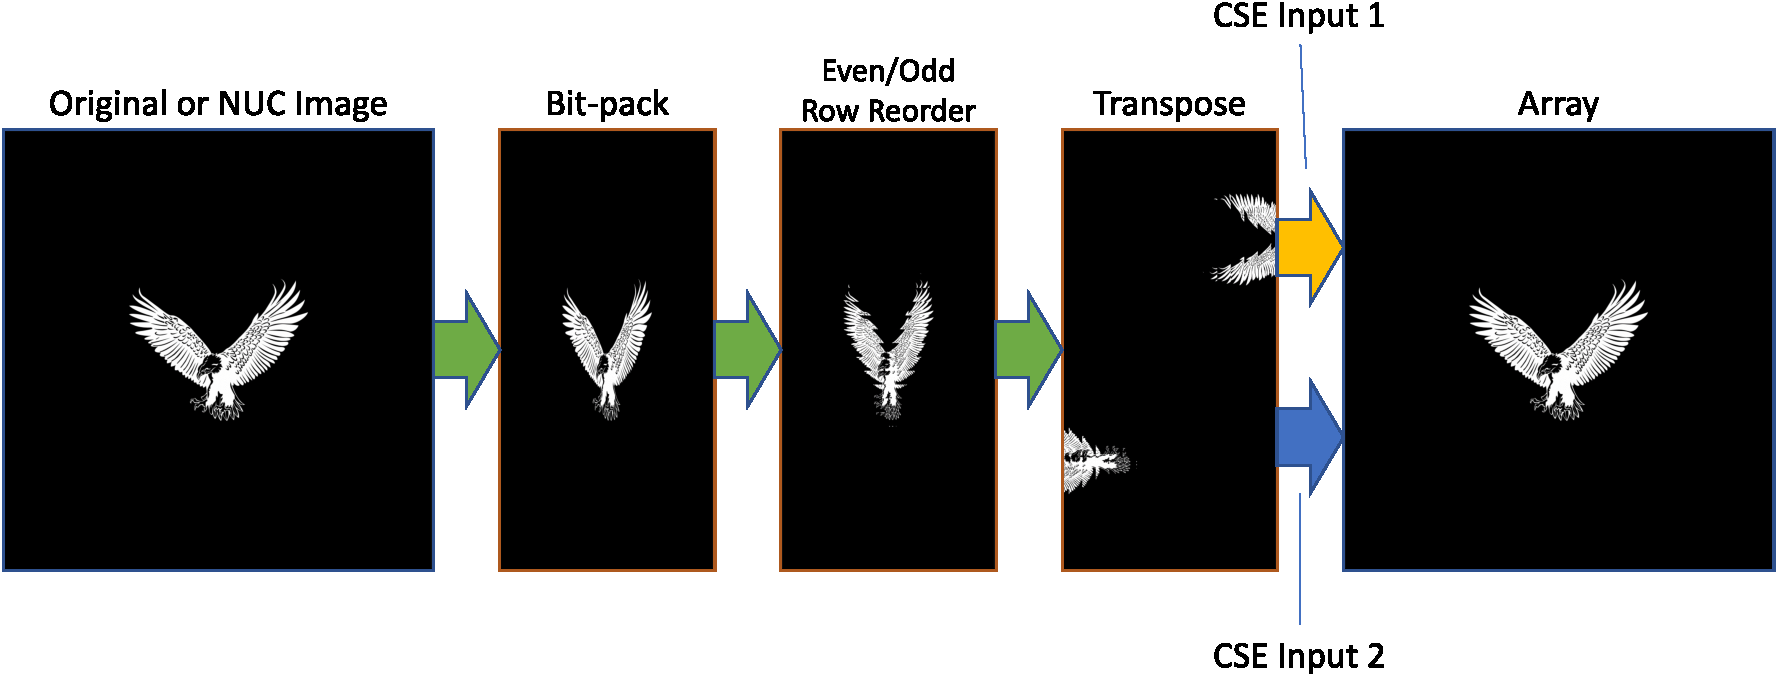
\includegraphics[width=1.0\textwidth]{fig/image_encoding_ir2.pdf}
        \caption{Image Encoding: IR Example 2}
        \label{fig:image_encoding_ir_example2}
    \end{figure}

    While this chapter discussed the internal details of how imagery received within the array is formatted and written to an array, Chapter~\ref{chap:display_protocols} shifts to a discussion of how imagery is sent to an array at the protocol level within an IRSP system while providing details of the limitations and challenges present there.
